\section{Related Work}

\begin{figure*}[t]
% \vspace{-0.15in}
  \centering
  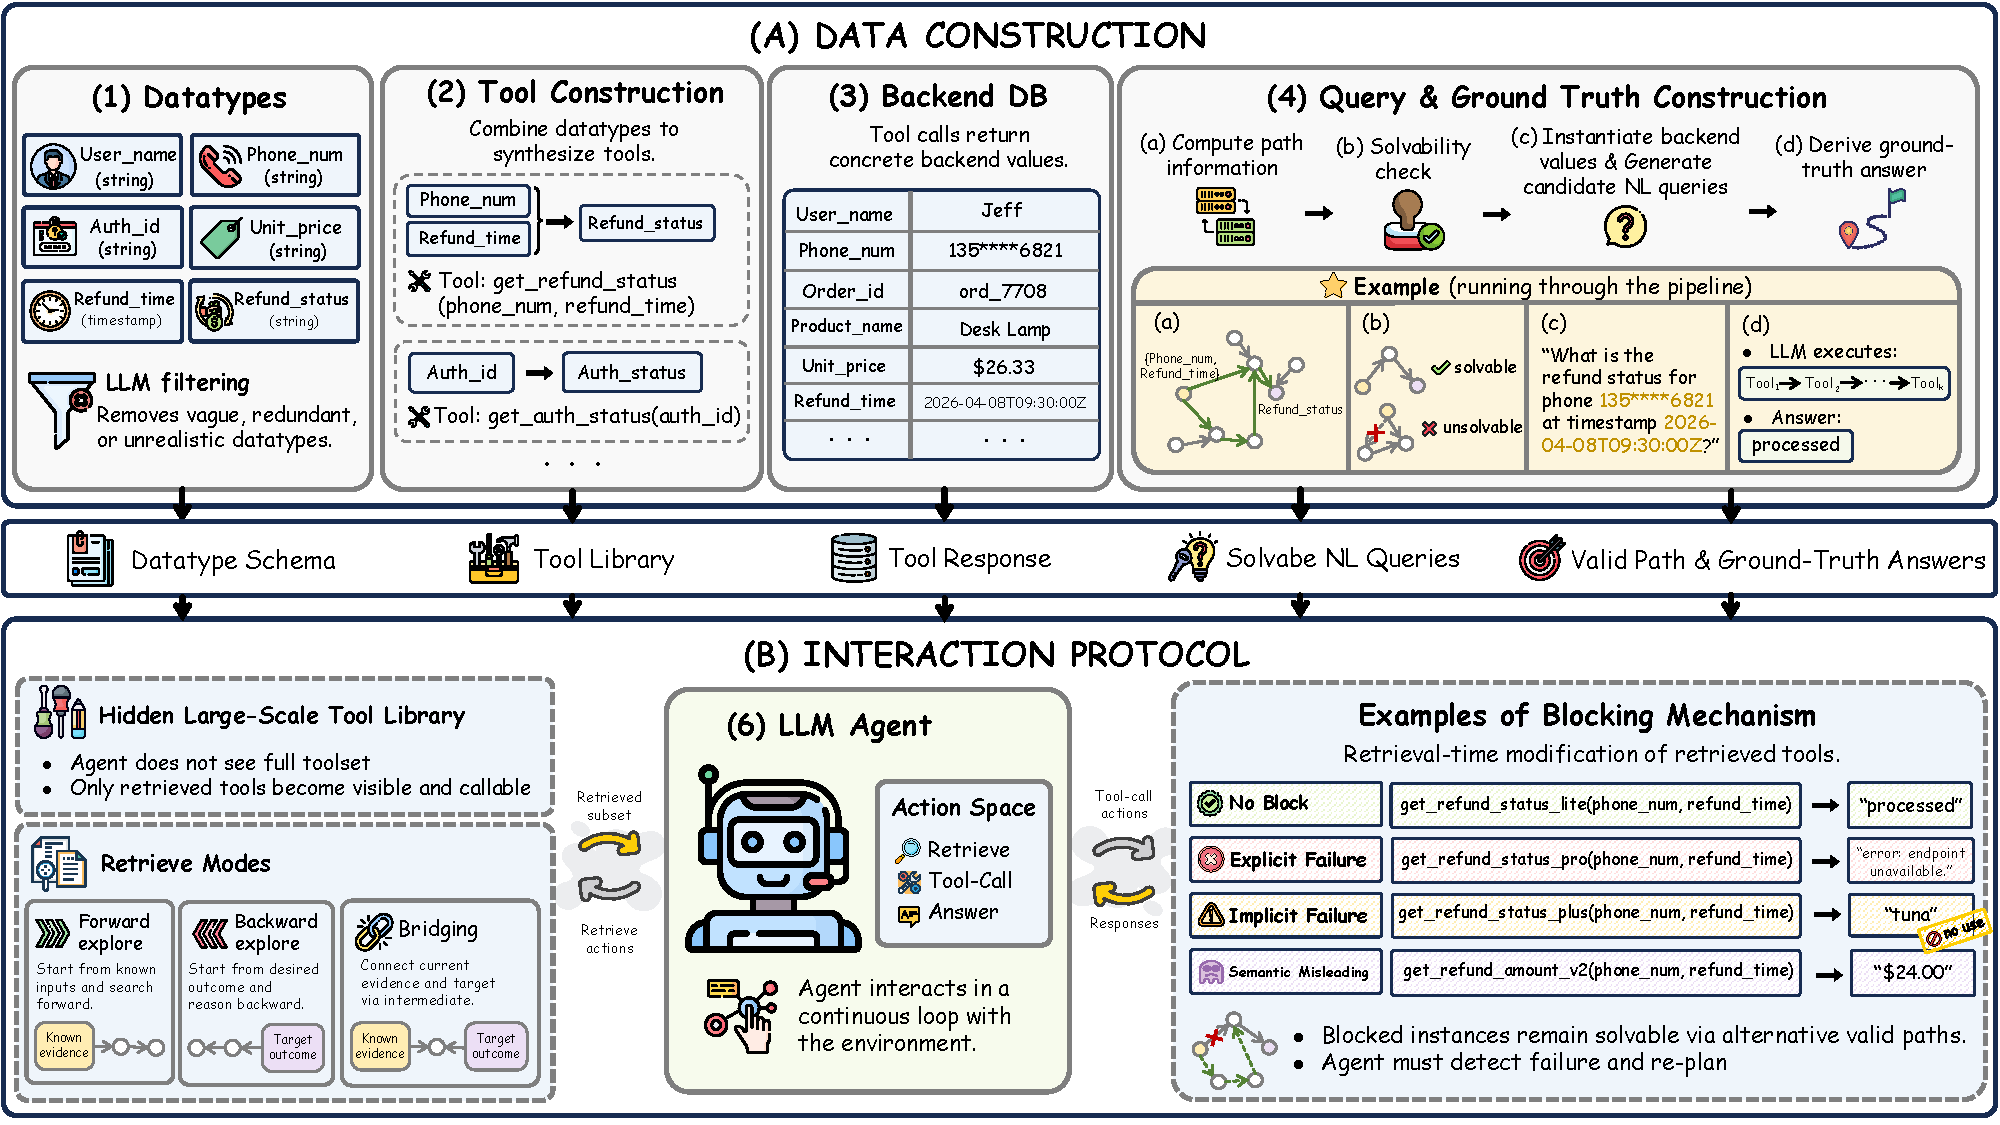
\includegraphics[width=1\linewidth]{Figures/demo_figure_pdf.pdf}
  \vspace{-0.25in}
  \caption{Overview of \bench{}. \textit{\textbf{Data construction}} turns typed retail datatypes into executable tools and backend records, then derives solvable queries with ground-truth answers. \textit{\textbf{Runtime protocol}} evaluates agents as they retrieve and invoke tools via bidirectional exploration, while retrieval-time blockers force re-planning.}
  \label{fig:demo_figure}
  \vspace{-0.15in}
\end{figure*}

\paragraph{Evaluating Agentic Planning with Large-Scale Toolsets.}

% Goal: Differentiate different benchmarks with our works
% 1. Planning over large-scale toolsets is central to complex agentic tasks, where agents must explore diverse tool-use paths and remain robust to noisy or unreliable tools.

% 2. Existing evaluations have studied agent exploration abilities and tool noise resilience in different aspects.

% 2.1 Discuss agent/tool-use benchmarks about planning with large-scale tools with implicit subgoals, which requires the agents to explore the intermediate goals.
% ~\citep{EscapeBench}

% 2.2 Discuss agent/tool-use benchmark about adaptive planning with unreliable tools, which requires the agents to adaptively plan and re-plan.

% 2.3 Discuss benchmarks that combines both, and point out their limitations. what previous works do not cover is implicit subgoals and lack of encouraging bidirectional exploration

% 3. One short sentence about our mitigation/novelty，aka how does our benchmark fills the gap

Planning over large-scale tool ecosystems is central to complex agentic tasks, where agents must compose multi-step tool-use trajectories while handling unreliable tool access. 
Existing benchmarks have examined this challenge from several perspectives. 
% \jy{do not claim parts of this problem, you could directly say that existing benchmarks discussed this problem in xxx way and cite the papers, then you could say their perspective is}
Large-scale tool-use and retrieval benchmarks evaluate tool selection over broad tool collections~\citep{ToolBench,APIBench,API-Bank,ToolRet,MCP-Bench,LiveMCPBench}, but often focus on relatively explicit task goals. 
Long-horizon benchmarks cover stateful execution~\citep{ToolSandbox}, multi-hop chaining~\citep{ToolHop}, implicit-goal solving~\citep{EscapeBench}, and extended workflows~\citep{Tool-Decathlon}, but generally assume available tools rather than unreliable, retrieval-mediated access.
Robustness-oriented benchmarks introduce noisy users~\citep{AgentNoiseBench,UserBench}, imperfect tools~\citep{OpaqueToolsBench,ToolQA-D}, or tool-state failures~\citep{ToolGym,CostBench}, but rarely combine adaptation with active search over large tool spaces. 
Thus, our benchmark evaluates adaptive planning under partial tool observability and unreliable tool availability, requiring agents to explore bi-directionally and adapt when tool-use paths are disrupted.

\paragraph{Agent Designs for Large-Scale Tool Planning.}

% Goal: Show that existing agent designs couldn't solve the problem, since we only test different LLM backbones instead of various agent architecture.
% Basically the idea is, list out what existing single agent framework / multi-agent systems emphasis on and group them together. The following will list out the steps to write this part.

% 1. Existing agentic designs have looked into the problem of planning with massive tool sets.
% 2. For single agent framework / harness, they do (1), (2), (3) things and thus focus on corresponding (1), (2), (3) ability.
% 3. While multi-agent systems also emerges due to the longevity as well as heavy cognitive load in this problem. One line of work incorporate (1) method in xxx (cite(1), (2), (3)), and thus solve xxx, while another line of work xxx (similarly)
% 4. Why our benchmark is challenging: why previous agent designs couldn't solve the problem

% \qh{add references}

Prior work has developed various agent designs for planning with large-scale tool ecosystems. 
Among them, some single-agent frameworks focus on modular tool invocation \citep{karpas2022mrkl, schick2023toolformer}, reasoning--acting control and long-horizon planning \citep{erdogan2025planact, ReAct, koh2025treesearch}, and scalable tool selection from large tool libraries \citep{AnyTool, ToolGen, AutoTool}. 
Multi-agent systems further reduce long-horizon cognitive load through communicative collaboration \citep{li2023camel, wu2024autogen, chen2024agentverse} and role- or workflow-based task decomposition \citep{hong2024metagpt, chen2025smurfs, ling2025elhplan}. 
However, even these designs primarily scaffold tool invocation, tool selection, and task decomposition, while leaving unresolved the core challenge posed by our benchmark: agents must actively explore implicit sub-goals and intermediate information, and then adaptively re-plan as observations emerge.



